\documentclass[twocolumn,preprintnumbers,amsmath,amssymb]{revtex4-2}
%\documentclass[preprint]{elsarticle}
\usepackage{amsmath}
\usepackage{amssymb}
\usepackage{graphicx}
\usepackage{float}
\usepackage[usenames,dvipsnames]{color}

\newcommand{\wt}[1]{\widetilde{#1}}
\newcommand{\eq}[1]{#1^{(eq)}}
\newcommand{\peq}[1]{#1^{'(eq)}}
\newcommand{\req}[1]{Eq.\,({\ref{#1}})}
\newcommand{\reqs}[2]{Eqs.\,({\ref{#1}}-{\ref{#2}})}
\newcommand{\reff}[1]{Fig.\,({\ref{#1}})}
\newcommand{\mk}{|\boldsymbol{k}|}
\newcommand{\ft}[1]{\widetilde{\boldsymbol{#1}}}
\newcommand{\CgNote}[1]{\textcolor{cyan}{#1}}
\begin{document}
%\preprint{Draft.13}
\title{Magnetic properties of finite temperature electron-positron plasma in the early universe}
\author{Cheng Tao Yang$^a$, Andrew Steinmetz$^a$, and Johann Rafelski$^a$}
\affiliation{$^a$ Department of Physics, The University of Arizona, Tucson, Arizona 85721, USA}


\date{\today}

%%%%%%%%%%%%%%%%%%%%%%%%%%%%%%%%%%%%%%%%%%%%%%%%%%%%%%%%%%%%%%%%%%

\begin{abstract}
We will write something here for the abstract.
\end{abstract}
\maketitle

%%%%%%%%%%%%%%%%%%%%%%%%%%%%%%%%%%%%%%%%%%%%%%%%%%%%%%%%%%%%%%%%%%%
\section{Introduction}

{\color{blue}(Brief introduction for ee-plasma)} In early universe after neutrinos decoupled  at temperature $T\approx2$ MeV and become free-streaming from the cosmic plasma, the cosmic plasma was dominated by electrons, positrons, and photons. 
 Fig.~\ref{Density_fig} shows this plasma existed until $T\approx20\ \mathrm{keV}$ such that BBN occurred within a rich electron-positron plasma~\cite{Chris:2023abc}. The electron-positron plasma is the last epoch the Universe contained a significant fraction of its content in antimatter. The electron-positron epoch of the early Universe was home to Big Bang Nucleosynthesis (BBN), the annihilation of most electrons and positrons reheating both the photon and neutrino fields, as well as setting the stage for the eventual recombination period which would generate the cosmic microwave background (CMB). The properties of the electron-positron $e^{\pm}$ plasma in the early Universe has not received appropriate attention in an era of precision BBN studies~\cite{Pitrou:2018cgg}. The presence of $e^{\pm}$ pairs before and during BBN has been acknowledged by Wang, Bertulani and Balantekin~\cite{Wang:2010px,Hwang:2021kno} over a decade ago. This however was before necessary tools were developed to explore the connection between electron and neutrino plasmas~\cite{Mangano:2005cc,Birrell:2012gg,Birrell:2014uka}.
%~Figure~~~~~~~~~~~~~~~~~~~~~~~~~~~~~~~~~~~~~~~~~~~~~~~~~`
\begin{figure}[h]
\centerline{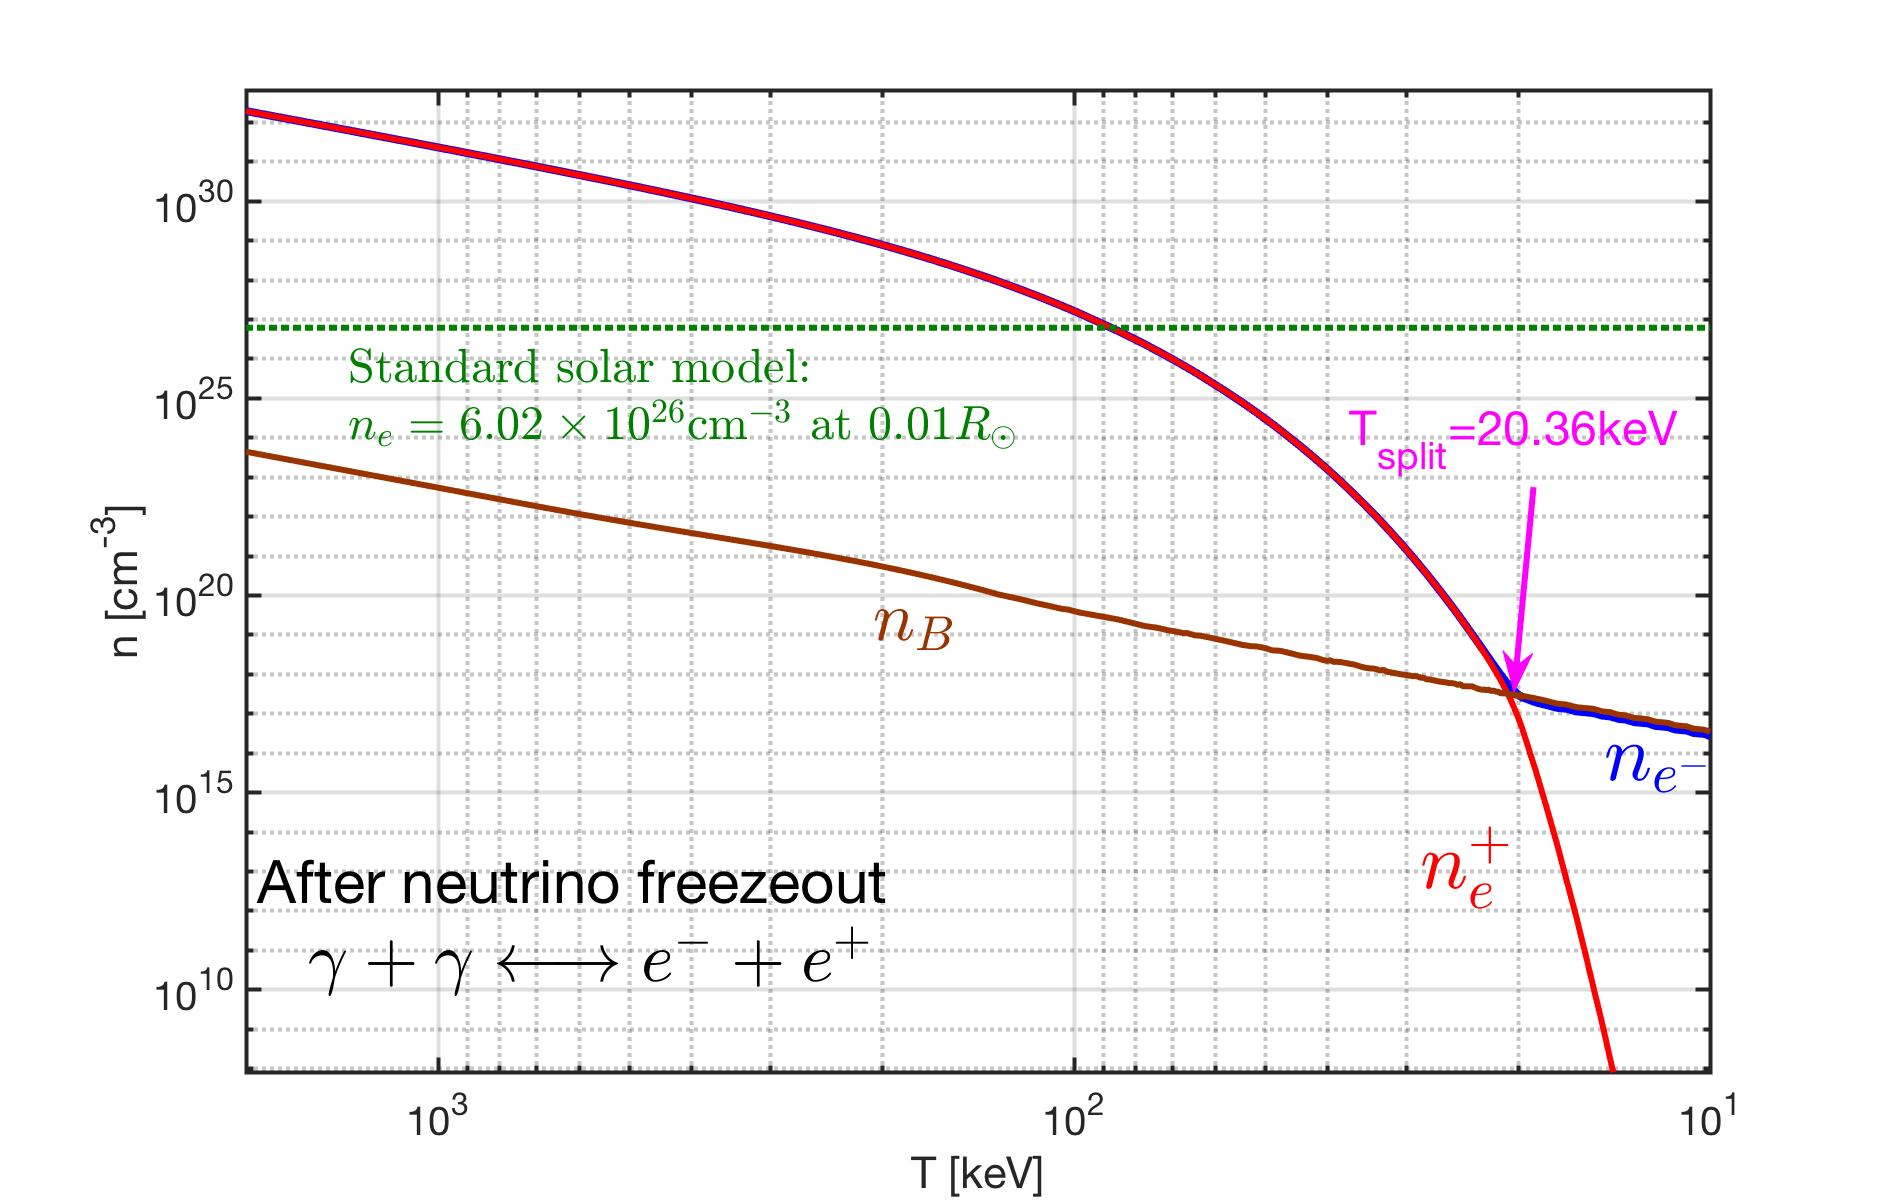
\includegraphics[width=0.5\textwidth]{./plots/NewDensity_cm3_new.jpg}}
\caption{The $e^{\pm}$ number densities as a function of temperature in the range $2\,\mathrm{MeV}>T>10\,\mathrm{keV}$. The blue solid line is the electron density $n_{e^{-}}$, the red solid line is the positron density $n_{e^{+}}$, and the brown solid line is the baryon density $n_{B}$. For comparison, we also show the green dotted line as the solar electron density within the solar core~\cite{Bahcall:2000nu}.}
\label{Density_fig} 
\end{figure}
%~~~~~~~~~~~~~~~~~~~~~~~~~~~~~~~~~~~~~~~~~~~~~~~~~~~~~~~~~

{\color{blue}(Brief introduction for magnetic field)} The Universe today filled with magnetic fields~\cite{Kronberg:1993vk} at various scales and strengths both within galaxies and in deep extra-galactic space far and away from matter sources. Extra-galactic magnetic fields are not well constrained today, but are required by observation to be non-zero~\cite{Anchordoqui:2001bs,Widrow:2002ud} with a magnitude between $10^{-12}\ \mathrm{T}>B_{EGMF}>10^{-20}\ \mathrm{T}$ over Mpc coherent length scales. The upper bound is constrained from the characteristics of the CMB while the lower bound is constrained by non-observation of ultra-energetic photons from blazars~\cite{Neronov:2010gir}. There are generally considered two possible origins~\cite{Widrow:2011hs,Vazza:2021vwy} for extra-galactic magnetic fields: (a) matter-induced dynamo processes involving Amperian currents and (b) primordial (or relic) seed magnetic fields whose origins may go as far back as the Big Bang itself. It is currently unknown which origin accounts for extra-galactic magnetic fields today or if it some combination of the two models. Even if magnetic fields in the Universe today are primarily driven via amplification through Amperian matter currents, such models still require primordial seed fields at some point to act as catalyst.
%~Figure~~~~~~~~~~~~~~~~~~~~~~~~~~~~~~~~~~~~~~~~~~~~~~~~~`
\begin{figure}[htbp]
 \centering 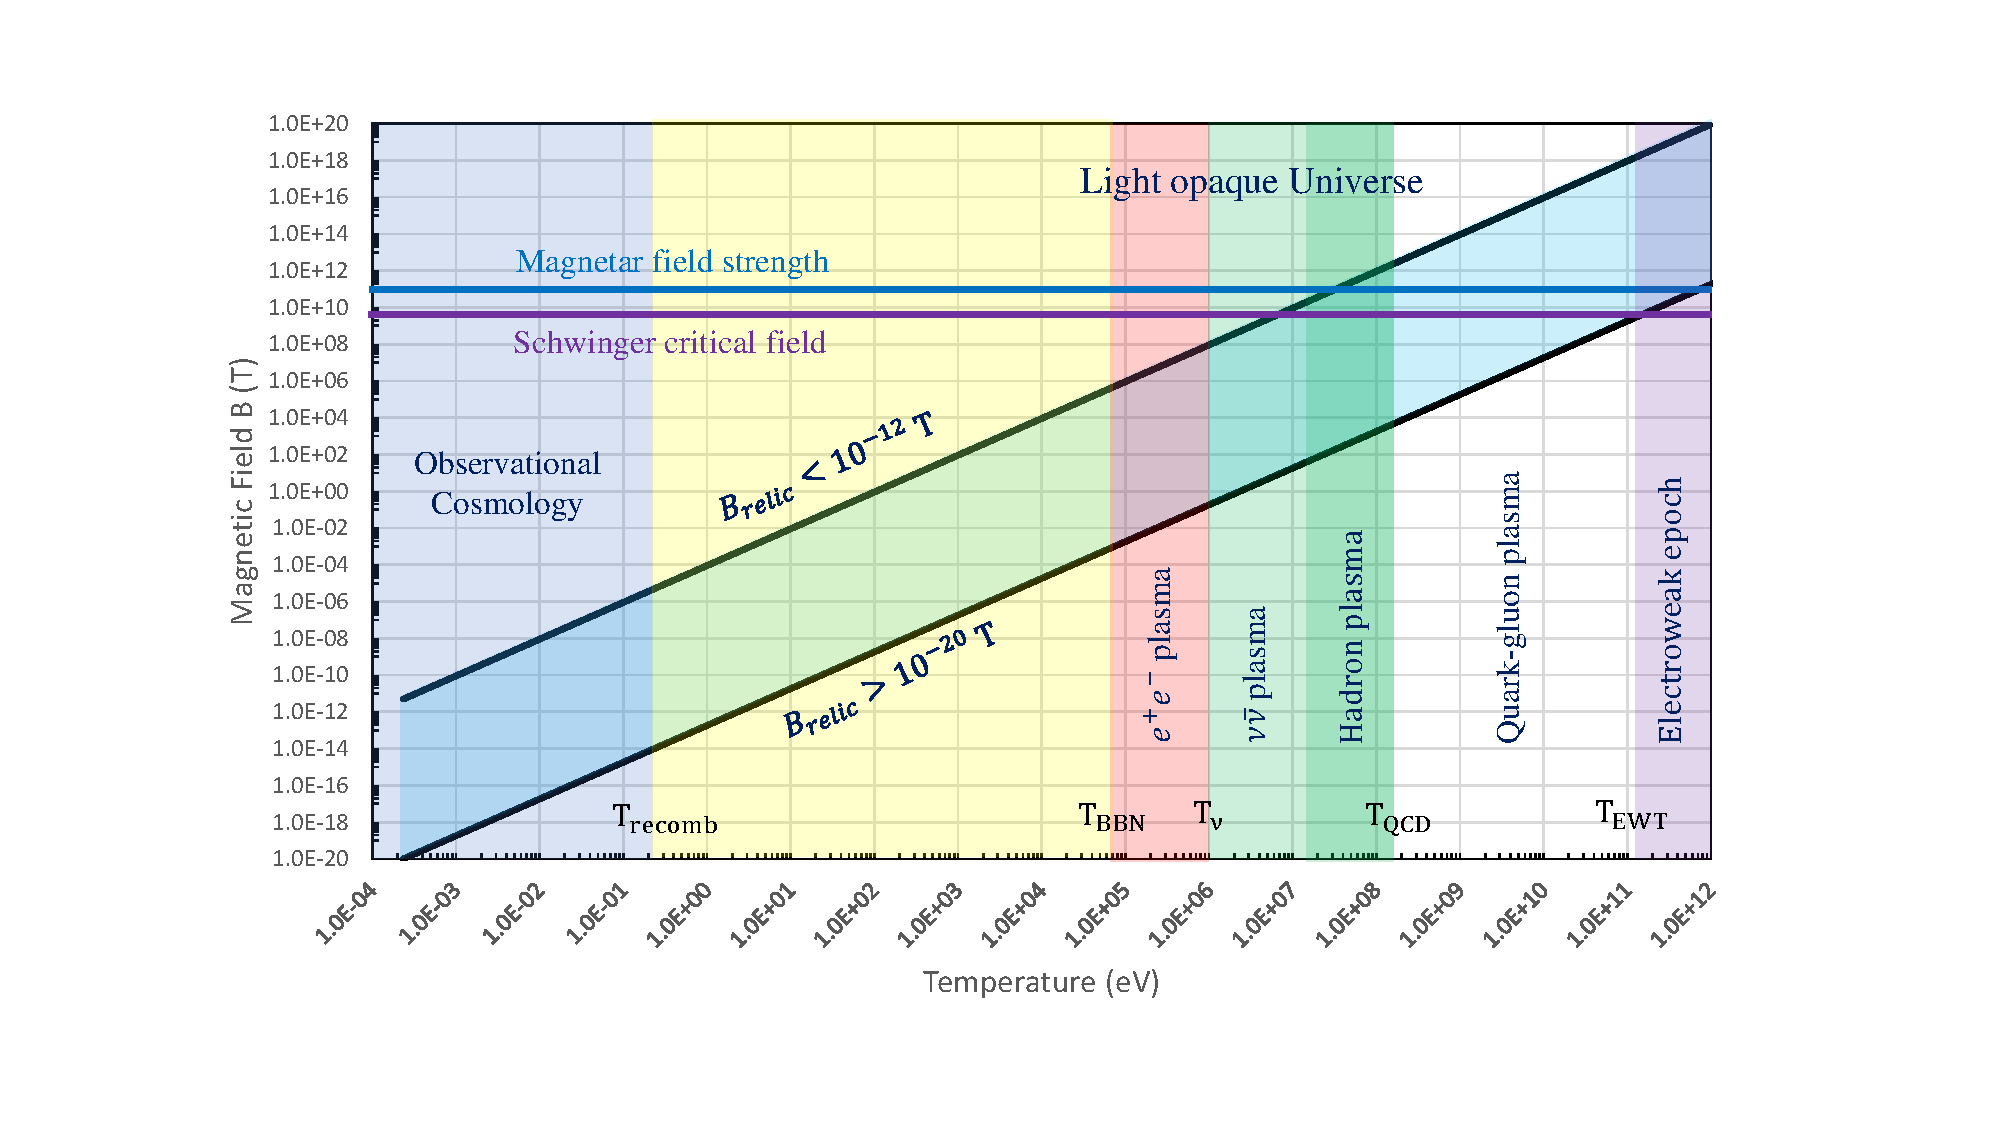
\includegraphics[trim=110 50 120 40,clip,width=0.5\textwidth]{./plots/relic_plot.pdf}
 \caption{Qualitative value of the primordial magnetic field over the evolutionary lifespan of the Universe. The upper and lower black lines represent extrapolation of the EGMF bounds into the past. The major phases of the Universe are indicated with shaded regions. The values of the Schwinger critical field (purple line) and the upper bound of surface magnetar field strength (blue line) are included for scale.\label{relic_plot}}
\end{figure}
%~~~~~~~~~~~~~~~~~~~~~~~~~~~~~~~~~~~~~~~~~~~~~~~~~~~~~~~~~

As the universe expand, the temperature cools as $T\propto1/a(t)$  and as magnetic flux is conserved over co-moving surfaces, we see in Fig.~\ref{relic_plot} that the primordial relic field is expected to dilute as $B\propto1/a(t)^{2}$. Motivated by these eredshit, we can introduce a dimensionless cosmic magnetic scale which is frozen in the homogeneous case as
\begin{alignat}{1}
 \label{Bo} b_{0}\equiv\frac{eB}{T^{2}}=\frac{eB\hbar c^{2}}{(k_{B}T)^{2}}\ \mathrm{(S.I)}\,,
\end{alignat}
where we've included the expression explicitly in full SI units. We can estimate the value of $b_{0}$ from the bounds of the extra-galactic magnetic field strength and the temperature of the Universe today. If the origin of deep space extra-galactic magnetic fields are relic fields from the early Universe, which today are expected to exist between $5\times10^{-12}\ \mathrm{T}>B_{relic}>10^{-20}\ \mathrm{T}$, then at temperature $T=2.7\ \mathrm{K}$, the value of the cosmic magnetic scale is between
\begin{alignat}{1}
 \label{BoScale} 5.5\times10^{-5}>b_{0}>1.1\times10^{-11}\,.
\end{alignat}
This should remain constant in the Universe at-large up to the last epoch the Universe was sufficiently magnetized to disturb this value. As the electron-proton plasma which generated the CMB was relatively dilute over its duration, it was unlikely sufficiently magnetized to significantly alter this value over extra-galactic scales. Rather, the best candidate plasma to have been sufficiently magnetized and dense to have set the relic field magnetic scale would have been the electron-positron plasma which existed during the duration of Big Bang Nucleosynthesis (BBN) and beforehand.

As $b_0$ is a constant of expansion, this means the contemporary small bounded values of $5\times10^{-12}\ \mathrm{T}>B_{relic}>10^{-20}\ \mathrm{T}$ (coherent over $\mathcal{O}(1\ \mathrm{Mpc})$ distances) may have once represented large magnetic fields in the early Universe. Assuming the electron-proton plasma between the CMB and electron-positron annihilation did not greatly disturbed it, we can calculate the remnant values at the temperature $T=50\ \mathrm{keV}$ (which takes place in the middle of BBN) with the expression
\begin{align}
 \label{BBNFields} B(T)=\frac{b_{0}}{e}T^{2}\,,
\end{align}
yielding a range of field strengths
\begin{align}
 \label{BBNRange} 2.3\times10^{5}\ \mathrm{T}>B(T=50\ \mathrm{keV})>4.6\times10^{-4}\ \mathrm{T}\,,
\end{align}
Therefore, correctly describing the dynamics of this $e^{\pm}$ plasma is of interest when considering modern cosmic mysteries such as the origin of extra-galactic magnetic fields (EGMF)~\cite{Anchordoqui:2001bs,Neronov:2010gir}. While most approaches tackle magnetized plasmas from the perspective of classical or semi-classical magneto-hydrodynamics (MHD)~\cite{berezhiani1992influence,berezhiani1995large,Schlickeiser:2018hzq}, our perspective is to demonstrate that fundamental quantum statistical analysis can lead to further insights on the behavior of magnetized plasmas.

%%%%%%%%%%%%%%%%%%%%%%%%%%%%%%%%%%%%%%%
\section{Landau eigen-energies in cosmology}\label{sec:Landau}
As a starting point, we consider the energy eigenvalues of charged fermions within a homogeneous magnetic field. Here, we have several choices: We could assume the typical Dirac energy eigenvalues with gyro-magnetic g-factor set to $g=2$. But as electrons, positrons and most plasma species have anomalous magnetic moments (AMM), we require a more complete model. Another option would be to modify the Dirac equation with a Pauli term~\cite{thaller2013dirac}, often called the Dirac-Pauli (DP) approach, via
\begin{align}
 \label{Pauli} \hat{H}_{\mathrm{AMM}} = -a\frac{e}{2m_{e}}\frac{\sigma_{\mu\nu}F^{\mu\nu}}{2}\,,
\end{align}
where $\sigma_{\mu\nu}$ is the spin tensor proportional to the commutator of the gamma matrices and $F^{\mu\nu}$ is the EM field tensor. For the duration of this work, we will remain in natural units $(\hbar=c=k_{B}=1)$ unless explicitly stated otherwise. The AMM is defined via g-factor as
\begin{align}
 \label{AMM} \frac{g}{2}=1+a\,.
\end{align}
This approach, while straightforward, would complicate the energies making analytic understanding and clarity difficult without a clear benefit. Modifying the Dirac equation with \req{Pauli} yields the following eigen-energies
\begin{align}
 \label{DPEnergy} E_{n}^{s}\vert_{DP}=\sqrt{\left(\sqrt{m_{e}^{2}+2eB\left(n+\frac{1}{2}-s\right)}-\frac{eB}{2m}(g-2)s\right)^{2}+p_{z}^{2}}
\end{align}
This model for the electron-positron plasma of the early Universe has been used in work such as Strickland et. al.~\cite{Strickland:2012vu}. Our work here is then in part a companion peice which compares and contrasts the DP model of fermions to our preferred model for the AMM via the Klein-Gordon-Pauli (KGP) equation given by
\begin{alignat}{1}
 \label{KGP} \left(\left(i\partial_{\mu}-eA_{\mu}\right)^{2}-m_{e}^{2}-e\frac{g}{2}\frac{\sigma_{\mu\nu}F^{\mu\mu}}{2}\right)\Psi=0\,.
\end{alignat}
We wish to emphasize, that each of the three above models (Dirac, DP, KGP) are distinct and have differing physical consequences and are not interchangeable which we explored in the context of hydrogen-like atoms in~\cite{Steinmetz:2018ryf}. Recent work done in~\cite{rafelski2023study} discuss the benefits of KGP over other approaches for $g\neq2$ from a quantum field theory perspective. Exploring the statistical behavior of KGP in a cosmological context can lead to new insights in magnetization which may be distinguished from pure $g=2$ behavior of the Dirac equation or the \emph{ad hoc} modification imposed by the Pauli term in DP. One major improvement of the KGP approach over the more standard DP approach is that the energies take eigenvalues which are mathematically similar to the Dirac energies. Considering the $e^\pm$ plasma in a uniform magnetic field $B$ pointing along the $z$-axis, the energy of $e^\pm$ fermions can be written as
\begin{align}
 \label{KGPEnergy} &E_{n}^{s}\!=\!\sqrt{p^2_z+\tilde{m}^2+2eBn},\,\,\,\,\tilde{m}^2=m^2_e+eB\left(1-gs\right),\\
 &s=\pm{1}/{2},\qquad n=0,1,2,3,\dots
\end{align}
where $n$ is the principle quantum number for the Landau levels and $s$ is the spin quantum number. Here we introduce a notion of effective mass $\tilde{m}$ which inherits the spin-specific part of the energy adding them to the mass. This convention is also generalizable to further non-minimal electromagnetic models with more exotic energy contributions such that we write a general replacement as
\begin{align}
 \label{MagMass} m_{e}^{2}\rightarrow\tilde{m}^2(B)\,.
\end{align}
This definition also pulls out the ground state Landau energy separating it from the remainder of the Landau tower of states. One restriction is that the effective mass must remain positive definite in our analysis thus we require
\begin{align}
 \label{MassLimit} \tilde{m}^2(B)=m^2_e+eB\left(1-gs\right)>0\,.
\end{align}
This condition fails under ultra-strong magnetic fields of order
\begin{align}
 \label{MagMassFail} B_{\mathrm{crit}}=\frac{m_{e}^{2}}{ea}=\frac{\mathcal{B}_{S}}{a}\approx3.8\times10^{12}\ \mathrm{T}\,,
\end{align}
where $\mathcal{B}_{S}$ is the Schwinger critical field strength. For electrons, this field strength is well above the window of magnetic field strengths of interest during the late $e^{\pm}$ epoch.

%~~~~~~~~~~~~~~~~~~~~~~~~~~~~~~~~~~~~~~~~~~~~~~~~~~~~~~~~~~

There is another natural scale for the magnetic field besides \req{MagMassFail} when considering the consequences of FLRW expansion on the $e^{\pm}$ fluid. As the Universe expands, different terms in the energies and thus partition function evolve as a function of the scale factor $a(t)$ which arises in the FLRW metric. We can consider the expansion to be an adiabatic process which results in a smooth shifting of the relevant dynamical quantities. From the conservation of magnetic flux through a co-moving surface, the magnetic field under expansion starting at some initial time $t_{0}$ is given by
\begin{alignat}{1}
 \label{BScale} B(t) = B(t_{0})\frac{a(t_{0})^{2}}{a(t)^{2}}\,.
\end{alignat}
As the Universe expands, the temperature also cools as the cosmological redshift reduces the momenta of particles in the Universe lowering their contribution to the energy content of the Universe. This cosmological redshift is written as
\begin{alignat}{1}
 \label{Redshift} p_{i}(t) = p_{i}(t_{0})\frac{a(t_{0})}{a(t)}\,,\qquad T(t) = T(t_{0})\frac{a(t_{0})}{a(t)}\,.
\end{alignat}
The momenta scale with the same factor as temperature as it is the origin of cosmological redshift. The energy of massive free particles in the Universe scales differently based on their momentum (and thus temperature). When hot and relativistic, particle energy scales with inverse scale factors like radiation. However as particles transition to non-relativistic momenta, their energies scale with the inverse square of the scale factor like magnetic flux.
\begin{alignat}{1}
 \label{EScale} E(t) = E(t_{0})\frac{a(t_{0})}{a(t)}\xrightarrow{\mathrm{NR}}\ E(t_{0})\frac{a(t_{0})^{2}}{a(t)^{2}}\,.
\end{alignat}
This occurs because of the functional dependence of energy on momentum in the relativistic versus non-relativistic cases. The argument in the Boltzmann statistical factor is given by
\begin{alignat}{1}
 \label{Boltz} X_{n}^{s}\equiv\frac{E_{n}^{s}}{T}\,.
\end{alignat}
We can explore this relationship for the magnetized system explicitly by writing out \req{Boltz} using the KGP eigen-energies as
\begin{alignat}{1}
 \label{XExplicit} X_{n}^{s} = \sqrt{\frac{m_{e}^{2}}{T^{2}}+\frac{p_{z}^{2}}{T^{2}}+\frac{2eB}{T^{2}}\left(n+\frac{1}{2}-\frac{gs}{2}\right)}\,,
\end{alignat}
where we now introduce the expansion scale factor via \req{BScale} - \req{Redshift}. The Boltzmann factor can then be written as
\begin{alignat}{1}
 \label{XScale} X_{n}^{s}[a(t)] = \sqrt{\frac{m_{e}^{2}}{T^{2}(t_{0})}\frac{a(t)^{2}}{a(t_{0})^{2}}+\frac{p_{z}^{2}(t_{0})}{T^{2}(t_{0})}+\frac{2eB(t_{0})}{T^{2}(t_{0})}\left(n+\frac{1}{2}-\frac{gs}{2}\right)}\,.
\end{alignat}
This reveals that only the mass contribution is dynamic over cosmological time. For any given eigen-state, the mass term increases driving the state into the non-relativistic limit while the momenta and magnetic contributions are frozen by initial conditions.



%%%%%%%%%%%%%%%%%%%%%%%%%%%%%%%%%%%%%%%
\section{Partition function for Electron-Positron plasma}\label{sec:Partition}
\noindent We now turn our attention now to the statistical behavior of the $e^{\pm}$ system. We can utilize the general fermion partition function given by~\cite{Elze:1980er}
\begin{align}
 \label{PartFunc} \ln\mathcal{Z}=\sum_{\alpha}\ln\left(1+e^{-\beta(E-\eta)}\right)\,,
\end{align}
where $\beta=1/T$, $\alpha$ is the set of all quantum numbers in the system, and $\eta$ is the generalized chemical potential. The magnetized $e^{\pm}$ system should be considered a system of four quantum species: Particles and antiparticles, and spin aligned and anti-aligned. Taken together we consider a system where all electrons and positrons are spin aligned or anti-aligned with the magnetic field $B$ and the partition function of the system is written as
\begin{align}\label{PartFuncB}
\ln\mathcal{Z}_{tot}=&\frac{2eBV}{(2\pi)^2}\sum_{\sigma}^{\pm1}\sum_{s}^{\pm1/2}\sum_{n=0}^\infty\notag\\
\qquad&\int^\infty_{0}dp_z\left[\ln\left(1+\Upsilon_{\sigma}^{s}(x)e^{-\beta E_{n}^{s}}\right)\right]\,
\end{align}
where the fugacity is defined as
\begin{align}\label{Fugacity}
\Upsilon_{\sigma}^{s}(x)=\gamma(x)\lambda_{\sigma}^{s}\,,\qquad\lambda_{\sigma}^{s}=e^{(\sigma\eta_{e}+s\eta_{s})/T}\,,
\end{align}
where $\eta_{e}$ is the electron chemical potential and $\eta_s$ is the spin chemical potential for the generalized fugacity $\lambda_{\sigma}^{s}$. The parameter $\gamma(x)$ is a spatial field which controls the distribution inhomogeneity of the Fermi gas. Inhomogeneities can arise from the influence of other forces on the gas such as gravitational forces. Deviations of $\gamma\neq1$ represent configurations of reduced entropy (maximum entropy yields the normal Fermi distribution itself with $\gamma=1$) without pulling the system off a thermal temperature. This situation is similar to that of the quarks during QGP, but instead here the deviation is spatial rather than in time. This is precisely the kind of behavior that may arise in the $e^{\pm}$ epoch as the dominant photon thermal bath keeps the Fermi gas in thermal equilibrium while spatial inequilibria could spontaneously develop. For the remainder of this work, we will retain $\gamma(x)=1$. The energy $E_{n}^\pm$ can be written as
\begin{align}
&E_{n}^\pm=\sqrt{p^2_z+\tilde m^2_\pm+2eBn},\\
&\tilde{m}^2_\pm=m^2_e+eB\left(1\mp\frac{g}{2}\right)\,,
\end{align}
where the $\pm$ script refers to spin aligned and anti-aligned eigenvalues. As the temperature domain we're interested is in the $T=50\ \mathrm{keV}$ range, we can take a semi-relativistic approach of the electron-positron plasma by considering the partition function obtained in the Boltzmann approximation. In following we considering the case $\eta_s/T\ll1$ for the first approximation and Boltzmann approximation for non-relativistic electrons and positrons.

Using the Euler-Maclaurin formula to replace the sum over Landau levels with an integration yielding
\begin{align}
\ln\mathcal{Z}_{tot}=\ln\mathcal{Z}_{free}+\ln\mathcal{Z}_B+\ln\mathcal{Z}_R\,,
\end{align}
where we define the partition functions as  
\begin{align}
 \label{FreePart}&\ln\mathcal{Z}_{free}=\frac{T^3V}{2\pi^2}\left[2\cosh{\left(\frac{\eta_{e}}{T}\right)}\right]\sum_{i=\pm}x_i^2K_2\left(x_i\right)\,,\qquad x_i=\frac{\tilde{m}_i}{T}\\
 \label{MagPart}&\ln\mathcal{Z}_B=\frac{eBTV}{2\pi^2}\left[2\cosh{\left(\frac{\eta_{e}}{T}\right)}\right]\sum_{i=\pm}\bigg[\frac{x_i}{2}K_1\left(x_i\right)+\frac{k^2b_0}{12}K_0\left(x_i\right)\bigg]\,,\\
 \label{ErrorPart}&\ln\mathcal{Z}_R=\frac{eBTV}{\pi^2}\left[2\cosh{\left(\frac{\eta_{e}}{T}\right)}\right]R.
\end{align}
where $R$ is the error remainder which is defined by integrals over Bernoulli polynomials.
While this would require further derivation to demonstrate explicitly, the benefit of the Euler-Maclaurin approach is if the error contribution remains finite or bound for the magnetized partition function, then a correspondence between the free Fermi partition function (with noticeably modified effective mass $\tilde{m}_{\pm}$) and the magnetized Fermi partition function can be established. The mismatch between the summation and integral in the Euler-Maclaurin formula would then encapsulate the immediate magnetic response and deviation from the free particle phase space. While we label $\ln(\mathcal{Z}_{free})$ in \req{FreePart} as the \lq\lq free\rq\rq\ partition function, this is not strictly true as this contribution to the overall partition function is a function of the effective mass we defined earlier in \req{MagMass}. When determining the magnetization of the quantum Fermi gas, derivatives of the magnetic field $B$ will not fully vanish on this first term which will resulting in an intrinsic magnetization which is distinct from the contribution from the ground state and mismatch between the quantized Landau levels and the continuum of the free momentum. Specifically, this free Fermi contribution represents the magnetization that arises from the spin magnetic energy rather than orbital contributions.

Assuming the error remainder $R$ is small and can be neglected, we can rewrite \req{FreePart} - \req{MagPart} obtaining
\begin{align}
 \label{lnZ}
&\ln\mathcal{Z}_{tot}\!=\!\frac{T^3V}{2\pi^2}\left[2\cosh\left(\frac{\eta_{e}}{T}\right)\right]\notag\\
 &\times\sum_{i=\pm}\left\{x_i^{2} K_2\left(x_i\right)+\frac{b_0}{2}x_iK_1\left(x_i\right)+\frac{b^2_0}{12}K_0\left(x_i\right)\right\}.
\end{align}
\req{lnZ} is a surprisingly compact expression containing only tractable functions and will be our working model for the remainder of the work. Note that the above does not take into consideration density inhomogeneities and is restricted to the domain where the plasma is well described as a Maxwell-Boltzmann distribution. With that said, we have not taken the non-relativistic expansion of the eigen-energies.

\subsection{Charge neutrality and chemical potential}
\noindent In this section, we are interested in exploring the chemical potential of dense electron-positron plasma in the early Universe under the hypothesis of charge neutrality and entropy conservation. We focus on the temperature interval at the post-BBN temperature range $20<T<50$ keV. The charge neutrality can be written as
\begin{align}
 \label{density_proton}
 \left(n_{e}-n_{\bar{e}}\right)= X_p\left(\frac{n_B}{s_{\gamma,\nu}}\right)\,s_{\gamma,\nu},\qquad X_p\equiv\frac{n_p}{n_B}
\end{align}
where $n_B$ is the number density of baryon, and the entropy density is obtained by considering the contribution of $e^\pm$ in entropy density is negligible compared to the photon and neutrino entropy density at post-BBN temperature $20\keV<T<50\keV$ because the low density $n_e\ll n_{\gamma,\nu}$. In general the entropy density can be written as~\cite{kolb1990early}
\begin{align}
&s=\frac{2\pi^2}{45}g_sT_\gamma^3,\\ &g_s=\sum_{i=boson}g_i\left(\frac{T_i}{T_\gamma}\right)^3+\frac{7}{8}\sum_{i=fermion}g_i\left(\frac{T_i}{T_\gamma}\right)^3
\end{align}
where $g_s$ is the effective degree of freedom that contribute to the entropy density. The parameters $X_p$ and $(n_B/s)$ can be determined by the observation, we have $X_p=0.878\pm0.015$~\cite{ParticleDataGroup:2022pth} and entropy-per-baryon ratio from Eq.(\ref{BdS}). 


The net number density of electron can be obtained by using the partition function of electron-positron plasma in Boltzmann limit \req{lnZ} as follow:
\begin{align}\label{NetElectron}
\left(n_e-n_{\bar e}\right)&=\frac{T}{V}\frac{\partial}{\partial \eta_{e}}\ln\mathcal{Z}_{tot}\notag\\
&=\frac{T^3}{2\pi^2}\left[2\sinh{(\eta_{e}/T)}\right]\notag\\&\sum_{i=\pm}\left[x_i^2K_2(x_i)+\frac{b_0}{2}x_i K_1(x_i)+\frac{b^2_0}{12}K_0(x_i)\right]
\end{align}
Substituting Eq.(\ref{NetElectron}) into the charge neutrality condition Eq.(\ref{density_proton}) we can solve the chemical potential of electron $\eta_e/T$ as follow:
\begin{align}\label{ChemicalPotential}
%\sinh{(\eta_{e}/T)}&=\frac{2\pi^2}{2T^3}\,\frac{X_p(n_B/s_{\gamma,\nu})s_{\gamma,\nu}}{\sum_{i=\pm}\left[x_i^2K_2(x_i)+\frac{b_0}{2}x_i K_1(x_i)+\frac{b^2_0}{12}K_0(x_i)\right]}
&\sinh{(\eta_{e}/T)}=\frac{2\pi^2}{2T^3}\,X_p\left(\frac{n_B}{s_{\gamma,\nu}}\right)s_{\gamma,\nu}\notag\\
&\!\!\times\!\!\left[\sum_{i=\pm}\left(x_i^2K_2(x_i)+\frac{b_0}{2}x_i K_1(x_i)+\frac{b^2_0}{12}K_0(x_i)\right)\right]^{-1}
%&\longrightarrow\frac{2\pi^2n_p}{2T^3}\,\frac{X_p(n_B/s_{\gamma,\nu})s_{\gamma,\nu}}{2x^2K_2(x)},\qquad x=m_e/T,\qquad \mathrm{for}\,\,b_0=0\label{ChemiticalPotential_000}
\end{align}
%\req{ChemiticalPotential_000} shows that for the case $b_0=0$, the chemical potential agrees with our earlier results~\cite{Chris:2023abc}.
In {\ref{chemical_fig}}, we solve \req{ChemicalPotential} numerically and plot the chemical potential as a function of temperature $T$. It shows that the chemical potential of electron is not sensitive to the magnetic field because the small value of $b_0=10^{-5}\sim10^{-11}$ in the temperature range we consider and can be neglected in the denominator of \req{ChemicalPotential}. 
%%%%%%%%%%%%%%%%%%%%%%%%%%%%%%%%%%%%%%%
\begin{figure}[ht]
%\begin{center}
\centering
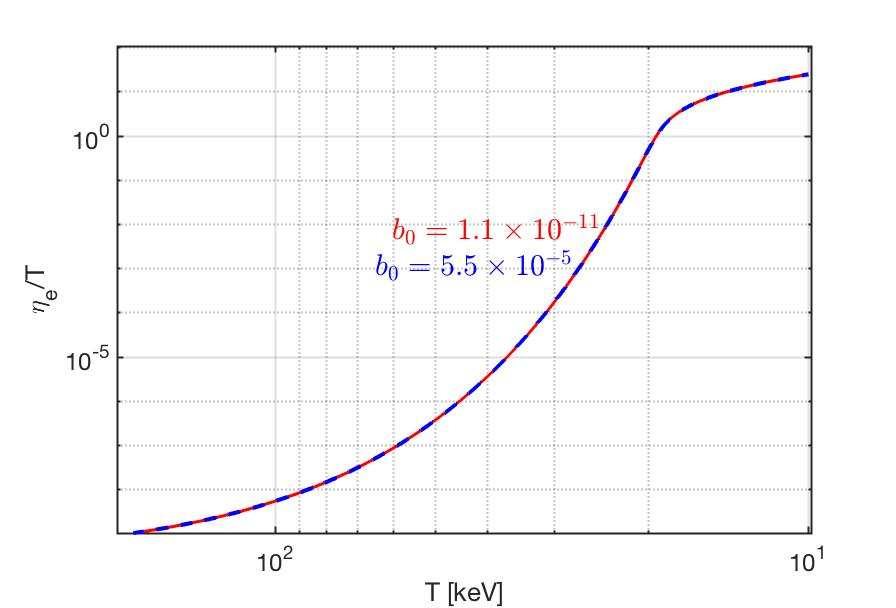
\includegraphics[width=0.5\textwidth]{./plots/ChemicalPotentialFinal_200keV.jpg}
\caption{The chemical potential $\eta_{e}/T$ a function of temperature $10<T<200$ keV. It shows that the chemical potential is not sensitive to the magnetic field $b_0$.}
\label{chemical_fig} 
\end{figure}
%%%%%%%%%%%%%%%%%%%%%%%%%%%%%%%%%%%%%%%

%%%%%%%%%%%%%%%%%%%%%%%%%%%%%%%%%%%%%%%
\subsection{Magnetization of the electron-positron plasma}\label{sec:Magnetization}
\noindent Considering the electron-positron partition function \req{lnZ} the magnetization can be obtained via the definition
\begin{align}
M=\frac{T}{V}\frac{\partial \ln\mathcal{Z}_{tot}}{\partial B}=\frac{T}{V}\left(\frac{\partial\tilde m_\pm}{\partial B}\right)\frac{\partial \ln\mathcal{Z}_{tot}}{\partial\tilde m_\pm}
\end{align}
It is convenient to rewrite the magnetization in dimensionless variable as follow
\begin{align}\label{Magnetization}
 \left(\frac{M}{B}\right)\!\!&=\!\!\frac{4\pi\alpha}{2\pi^2b_0}\left[2\cosh\left(\frac{\eta_{e}}{T}\right)\right]\notag\\
 &\times\sum_{i=\pm}\left\{c_{1}(x_{i})K_1(x_i)+c_{0}K_0(x_i)\right\}\,,
 \end{align}
 where the coefficients $c_1$ and $c_0$ are defined as
 \begin{align}
&c_{1}(x_{i})=\left[\frac{1}{2}-\left(\frac{1}{2}+\frac{ig}{4}\right)\left(1+\frac{b^2_0}{12x^2_i}\right)\right]x_i\,,\\
&c_{0} = \left[\frac{1}{6}-\left(\frac{1}{4}-\frac{ig}{8}\right)\right]b_0\,.
\end{align}
%%%%%%%%%%%%%%%%%%%%%%%%%%%%%%%%%%%%%%%
\begin{figure}[b]
%\begin{center}
\centering
%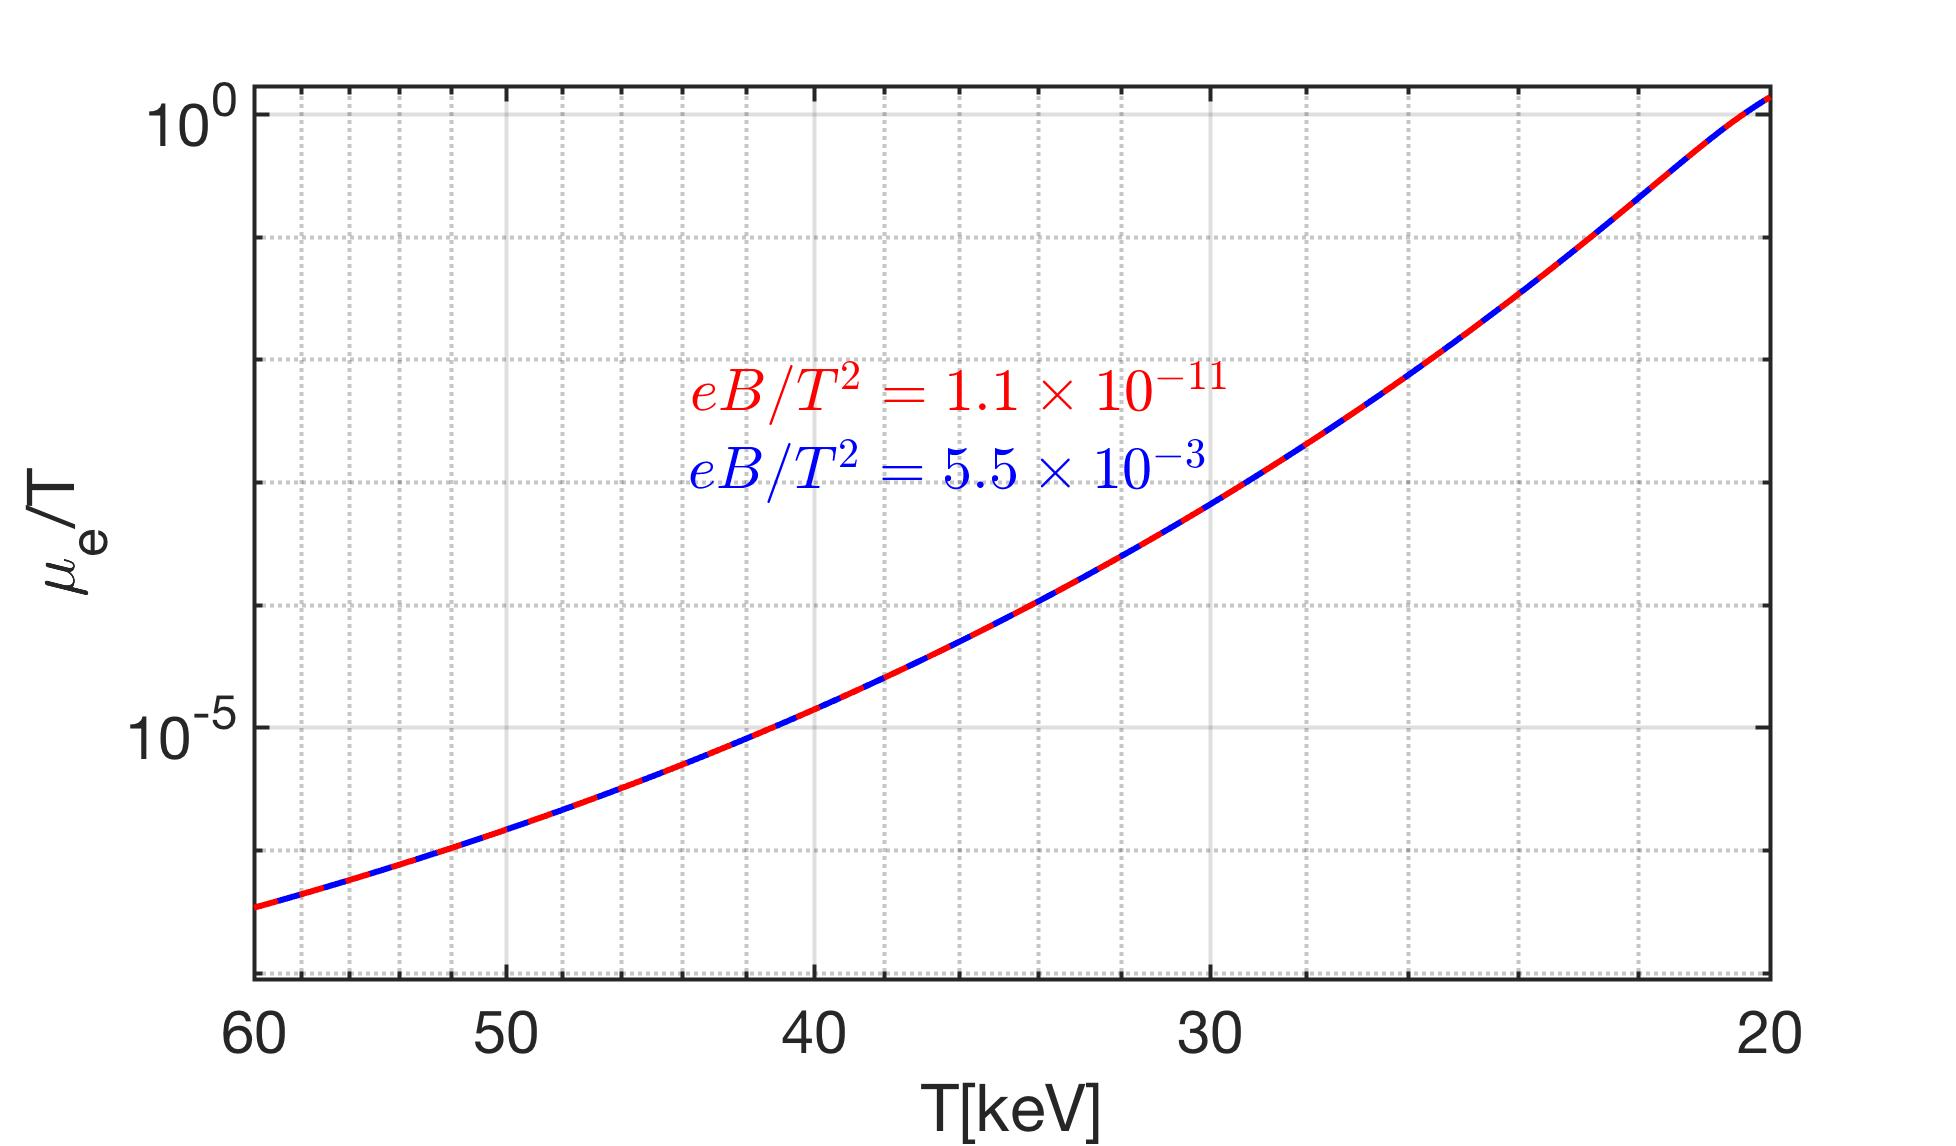
\includegraphics[width=0.75\linewidth]{./plots/ChemicalPotential_case2.jpg}
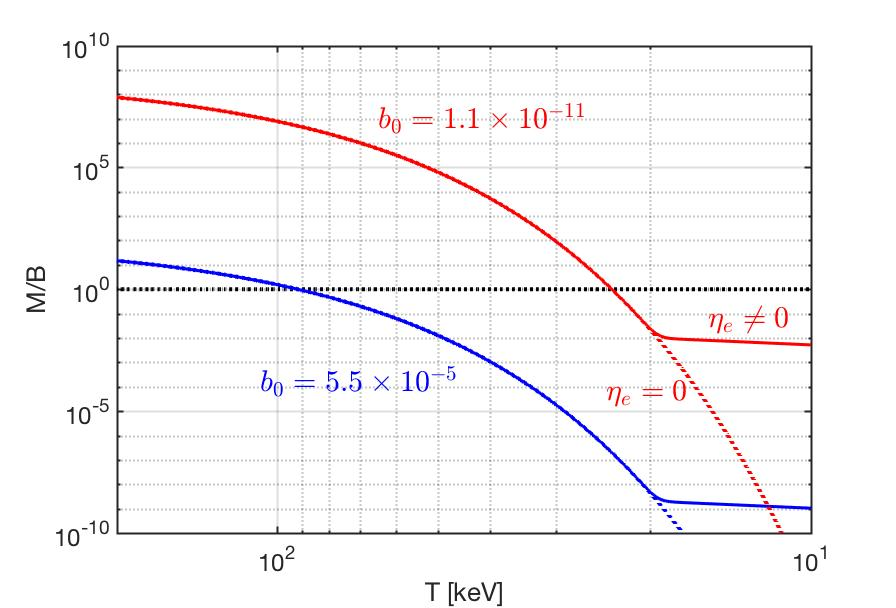
\includegraphics[width=0.5\textwidth]{./plots/MagnetizationFinal_200keV.jpg}
\caption{The magnetization $M/B$ as a function of temperature $10<T<200$ keV, where the solid line represent the case $\eta_e\neq0$ and dotted lines label the case $\eta_e=0$. It shows that for giving $b_0$ we can find the temperature that $M/B>1$ in early Universe.}
\label{Case2_fig} 
\end{figure}
%%%%%%%%%%%%%%%%%%%%%%%%%%%%%%%%%%%%%%%
Substituting the chemical potential \req{ChemicalPotential} into \req{Magnetization} we can solve the magnetization $M/B$ numerically.
Considering the case $g=2$ the magnetization can be written as 
\begin{align}
\left(\frac{M}{B}\right)=\left(\frac{M}{B}\right)_++\left(\frac{M}{B}\right)_-
\end{align}
where the functions $(M/B)_\pm$ are defined as 
\begin{itemize}
 \item Case1: $\tilde m_+=\sqrt{m^2_e+2eB}$, and $x_+=\tilde m_+/T$. The magnetization is given by
\begin{align}\label{Magnetization_001}
 &\left(\frac{M}{B}\right)_+\!\!=-\frac{8\pi\alpha}{2\pi^2}\sqrt{1+\sinh^2(\eta_e/T)}\notag\\
 &\times\left[\left(\frac{1}{2b_0}+\frac{b_0}{12x_+^2}\right)x_+K_1(x_+)+\frac{1}{3}K_0(x_+)\right]
\end{align}
 \item Case 2: $\tilde m_-=m_e$ and $x=\tilde m_-/T$,then the magnetization of electron/ positron becomes
\begin{align}\label{Magnetization_002}
&\left(\frac{M}{B}\right)_-\!\!=\frac{8\pi\alpha}{2\pi^2}\sqrt{1+\sinh^2(\eta_e/T)}\notag\\
&\qquad\qquad\times\left(\frac{1}{b_0}x_-K_1(x_-)+\frac{1}{6}K_0(x_-)\right)
\end{align}
\end{itemize}
Using the magnetic field $b_0$ and chemical potential $\eta_e/T$ we solve the magnetization numerically. In \ref{Case2_fig}, we plot the magnetization $M/B$ as a function of temperature $T$ showing that the magnetization depends on the magnetic field $b_0$ strongly. This is because for a small magnetic field $b_0$ the dominant term in \req{Magnetization_001} and \req{Magnetization_002} is $xK_1(x)/b_0$. For given $b_0$, the value of magnetization can be larger than the magnetic field, i.e. $M/B>1$ which shows the possibility that magnetic domains can be formed in the early Universe.



%%%%%%%%%%%%%%%%%%%%%%%%%%%%%%%%%%%%%%%%%%%%%%%%%%%%%%%%%%%%%%%%%%

%%%%%%%%%%%%%%%%%%%%%%%%%%%%%%%%%%%%%%%%%%%%%%%%%%%%%%%%%%%%%%%%%%%%%%
\begin{thebibliography}{99}
\end{thebibliography}
%%%%%%%%%%%%%%%%%%%%%%%%%%%%%%%%%%%%%%%%%%%%%%%%%%%%%%%%%%%%%%%%%%%
\end{document} 